

\tikzset{every picture/.style={line width=0.75pt}} %set default line width to 0.75pt        

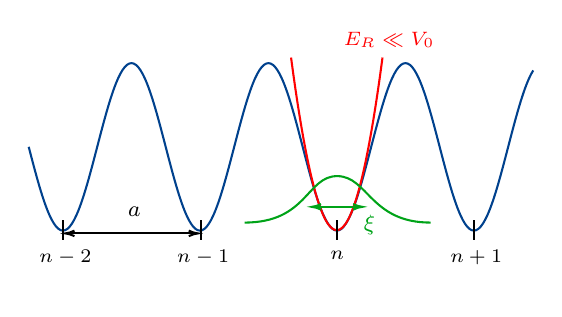
\begin{tikzpicture}[x=0.75pt,y=0.75pt,yscale=-1,xscale=1]
%uncomment if require: \path (0,135); %set diagram left start at 0, and has height of 135

%Shape: Wave [id:dp5948468038024646] 
\draw  [color={rgb, 255:red, 0; green, 65; blue, 141 }  ,draw opacity=1 ] (12,69.53) .. controls (17.38,90.2) and (22.53,109.88) .. (28.5,109.88) .. controls (34.47,109.88) and (39.62,90.2) .. (45,69.53) .. controls (50.38,48.86) and (55.53,29.18) .. (61.5,29.18) .. controls (67.47,29.18) and (72.62,48.86) .. (78,69.53) .. controls (83.38,90.2) and (88.53,109.88) .. (94.5,109.88) .. controls (100.47,109.88) and (105.62,90.2) .. (111,69.53) .. controls (116.38,48.86) and (121.53,29.18) .. (127.5,29.18) .. controls (133.47,29.18) and (138.62,48.86) .. (144,69.53) .. controls (149.38,90.2) and (154.53,109.88) .. (160.5,109.88) .. controls (166.47,109.88) and (171.62,90.2) .. (177,69.53) .. controls (182.38,48.86) and (187.53,29.18) .. (193.5,29.18) .. controls (199.47,29.18) and (204.62,48.86) .. (210,69.53) .. controls (215.38,90.2) and (220.53,109.88) .. (226.5,109.88) .. controls (232.47,109.88) and (237.62,90.2) .. (243,69.53) .. controls (247.01,54.12) and (250.9,39.25) .. (255.09,32.69) ;
%Shape: Parabola [id:dp32380929671166225] 
\draw  [color={rgb, 255:red, 255; green, 0; blue, 0 }  ,draw opacity=1 ] (138.4,26.5) .. controls (153.08,137.41) and (167.77,137.41) .. (182.45,26.5) ;
%Straight Lines [id:da20114798739595108] 
\draw    (31.67,111.22) -- (91.49,111.22) ;
\draw [shift={(93.49,111.22)}, rotate = 180] [color={rgb, 255:red, 0; green, 0; blue, 0 }  ][line width=0.75]    (4.37,-1.32) .. controls (2.78,-0.56) and (1.32,-0.12) .. (0,0) .. controls (1.32,0.12) and (2.78,0.56) .. (4.37,1.32)   ;
\draw [shift={(29.67,111.22)}, rotate = 0] [color={rgb, 255:red, 0; green, 0; blue, 0 }  ][line width=0.75]    (4.37,-1.32) .. controls (2.78,-0.56) and (1.32,-0.12) .. (0,0) .. controls (1.32,0.12) and (2.78,0.56) .. (4.37,1.32)   ;
%Straight Lines [id:da9743703357911851] 
\draw    (28.4,105) -- (28.4,114.51) ;

%Straight Lines [id:da7045788488223218] 
\draw    (94.8,105) -- (94.8,114.51) ;

%Straight Lines [id:da9576353190403918] 
\draw    (226.4,105) -- (226.4,114.51) ;

%Straight Lines [id:da19564966071273038] 
\draw    (160.4,105) -- (160.4,114.51) ;
%Curve Lines [id:da7613317075373456] 
\draw [color={rgb, 255:red, 0; green, 163; blue, 24 }  ,draw opacity=1 ]   (116,106) .. controls (146.29,106.02) and (145.91,83.51) .. (160.69,83.62) .. controls (175.46,83.73) and (176.69,106.02) .. (205.6,106) ;
%Straight Lines [id:da49305309064742076] 
\draw [color={rgb, 255:red, 0; green, 163; blue, 24 }  ,draw opacity=1 ]   (150.47,98.42) -- (170.69,98.42) ;
\draw [shift={(172.69,98.42)}, rotate = 180] [color={rgb, 255:red, 0; green, 163; blue, 24 }  ,draw opacity=1 ][line width=0.75]    (4.37,-1.32) .. controls (2.78,-0.56) and (1.32,-0.12) .. (0,0) .. controls (1.32,0.12) and (2.78,0.56) .. (4.37,1.32)   ;
\draw [shift={(148.47,98.42)}, rotate = 0] [color={rgb, 255:red, 0; green, 163; blue, 24 }  ,draw opacity=1 ][line width=0.75]    (4.37,-1.32) .. controls (2.78,-0.56) and (1.32,-0.12) .. (0,0) .. controls (1.32,0.12) and (2.78,0.56) .. (4.37,1.32)   ;

% Text Node
\draw (58.4,97) node [anchor=north west][inner sep=0.75pt]  [font=\footnotesize]  {$a$};
% Text Node
\draw (15.6,117.89) node [anchor=north west][inner sep=0.75pt]  [font=\scriptsize]  {$n-2$};
% Text Node
\draw (82,117.89) node [anchor=north west][inner sep=0.75pt]  [font=\scriptsize]  {$n-1$};
% Text Node
\draw (213.6,117.89) node [anchor=north west][inner sep=0.75pt]  [font=\scriptsize]  {$n+1$};
% Text Node
\draw (155.8,118.09) node [anchor=north west][inner sep=0.75pt]  [font=\scriptsize]  {$n$};
% Text Node
\draw (162.4,12.6) node [anchor=north west][inner sep=0.75pt]  [font=\scriptsize,color={rgb, 255:red, 255; green, 0; blue, 0 }  ,opacity=1 ]  {$E_{R} \ll V_{0}$};
% Text Node
\draw (172,101) node [anchor=north west][inner sep=0.75pt]  [font=\footnotesize,color={rgb, 255:red, 0; green, 163; blue, 24 }  ,opacity=1 ]  {$\xi $};


\end{tikzpicture}
